% ============================================================================
%  CHAPITRE 6 -- RÉSULTATS ET ANALYSE
% ============================================================================
\chapter{Résultats et analyse}
\label{chap:resultats}

Tous les chiffres proviennent de \srcfile{results/eval/}. Sauf mention contraire : $k/n = 1/12$, canal AWGN.

\section{CIFAR-10 : le résultat central}
\label{sec:res_cifar}

\begin{table}[H]
\centering
\caption{CIFAR-10, $k/n = 1/12$, AWGN. Référence : 88,4\,\% sur images originales.}
\label{tab:cifar}
\small
\begin{tabular}{@{}llrrr@{}}
\toprule
\textbf{SNR} & \textbf{Système} & \textbf{PSNR (dB)} & \textbf{SSIM} & \textbf{Précision} \\
\midrule
\multirow{4}{*}{\SI{0}{\decibel}}
 & JSCC syntaxique            & 20,08 & 0,669 & 42,0\,\% \\
 & \textbf{JSCC sémantique}   & \textbf{19,68} & \textbf{0,677} & \textbf{56,4\,\%} \\
 & Séparé — borne de capacité & 19,65 & 0,600 & 15,3\,\% \\
 & Séparé — meilleur MCS      & 12,63 & 0,132 & 9,8\,\% \\
\midrule
\multirow{4}{*}{\SI{10}{\decibel}}
 & JSCC syntaxique            & 25,99 & 0,874 & 67,6\,\% \\
 & \textbf{JSCC sémantique}   & \textbf{25,48} & \textbf{0,874} & \textbf{78,2\,\%} \\
 & Séparé — borne de capacité & 24,51 & 0,808 & 29,7\,\% \\
 & Séparé — meilleur MCS      & 19,65 & 0,600 & 15,3\,\% \\
\midrule
\multirow{4}{*}{\SI{20}{\decibel}}
 & JSCC syntaxique            & 27,72 & 0,906 & 70,6\,\% \\
 & \textbf{JSCC sémantique}   & \textbf{27,15} & \textbf{0,903} & \textbf{80,2\,\%} \\
 & Séparé — borne de capacité & 27,33 & 0,896 & 67,4\,\% \\
 & Séparé — meilleur MCS      & 25,71 & 0,850 & 40,5\,\% \\
\bottomrule
\end{tabular}
\end{table}

\begin{enumerate}
  \item \textbf{Le compromis sémantique est constant} : $\approx$\SI{0.5}{\decibel} de PSNR cédé, 10 à
        14~points de précision gagnés, à tous les SNR, sans dégradation du SSIM. Les pixels sacrifiés
        n'étaient pas ceux qui portaient le sens.
  \item \textbf{L'effet falaise est massif} : à \SI{0}{\decibel}, la chaîne séparée réelle donne 9,8\,\%, le
        niveau du hasard sur dix classes, contre 42\,\% et 56,4\,\% pour les systèmes appris.
  \item \textbf{La borne idéale est dépassée en précision} : elle ne corrige pas le \emph{critère}, son
        codeur de source optimisant toujours la fidélité pixel.
\end{enumerate}

\begin{figure}[H]
  \centering
  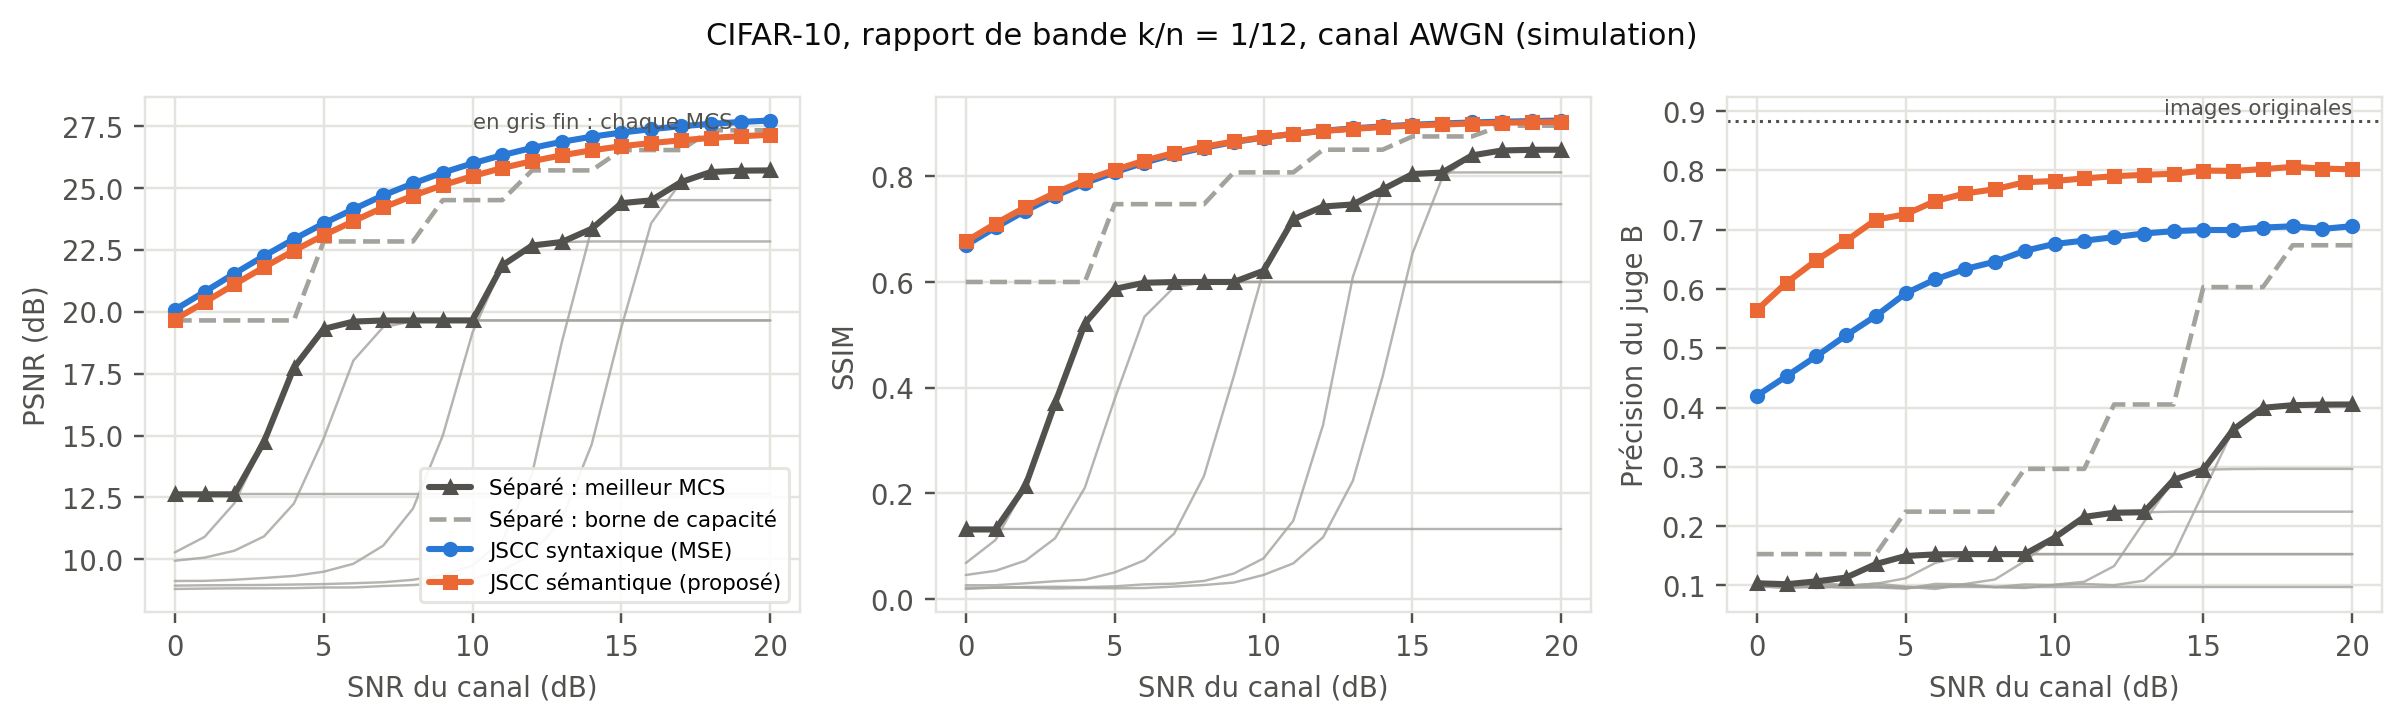
\includegraphics[width=0.80\linewidth]{cifar_snr.png}
  \caption{CIFAR-10 à $k/n = 1/12$ en fonction du SNR. Les courbes fines sont les MCS fixes de la chaîne
  séparée : leur plafonnement puis leur effondrement est l'effet falaise.}
  \label{fig:cifar_snr}
\end{figure}

\section{Influence du rapport de bande}
\label{sec:res_bande}

\begin{figure}[H]
  \centering
  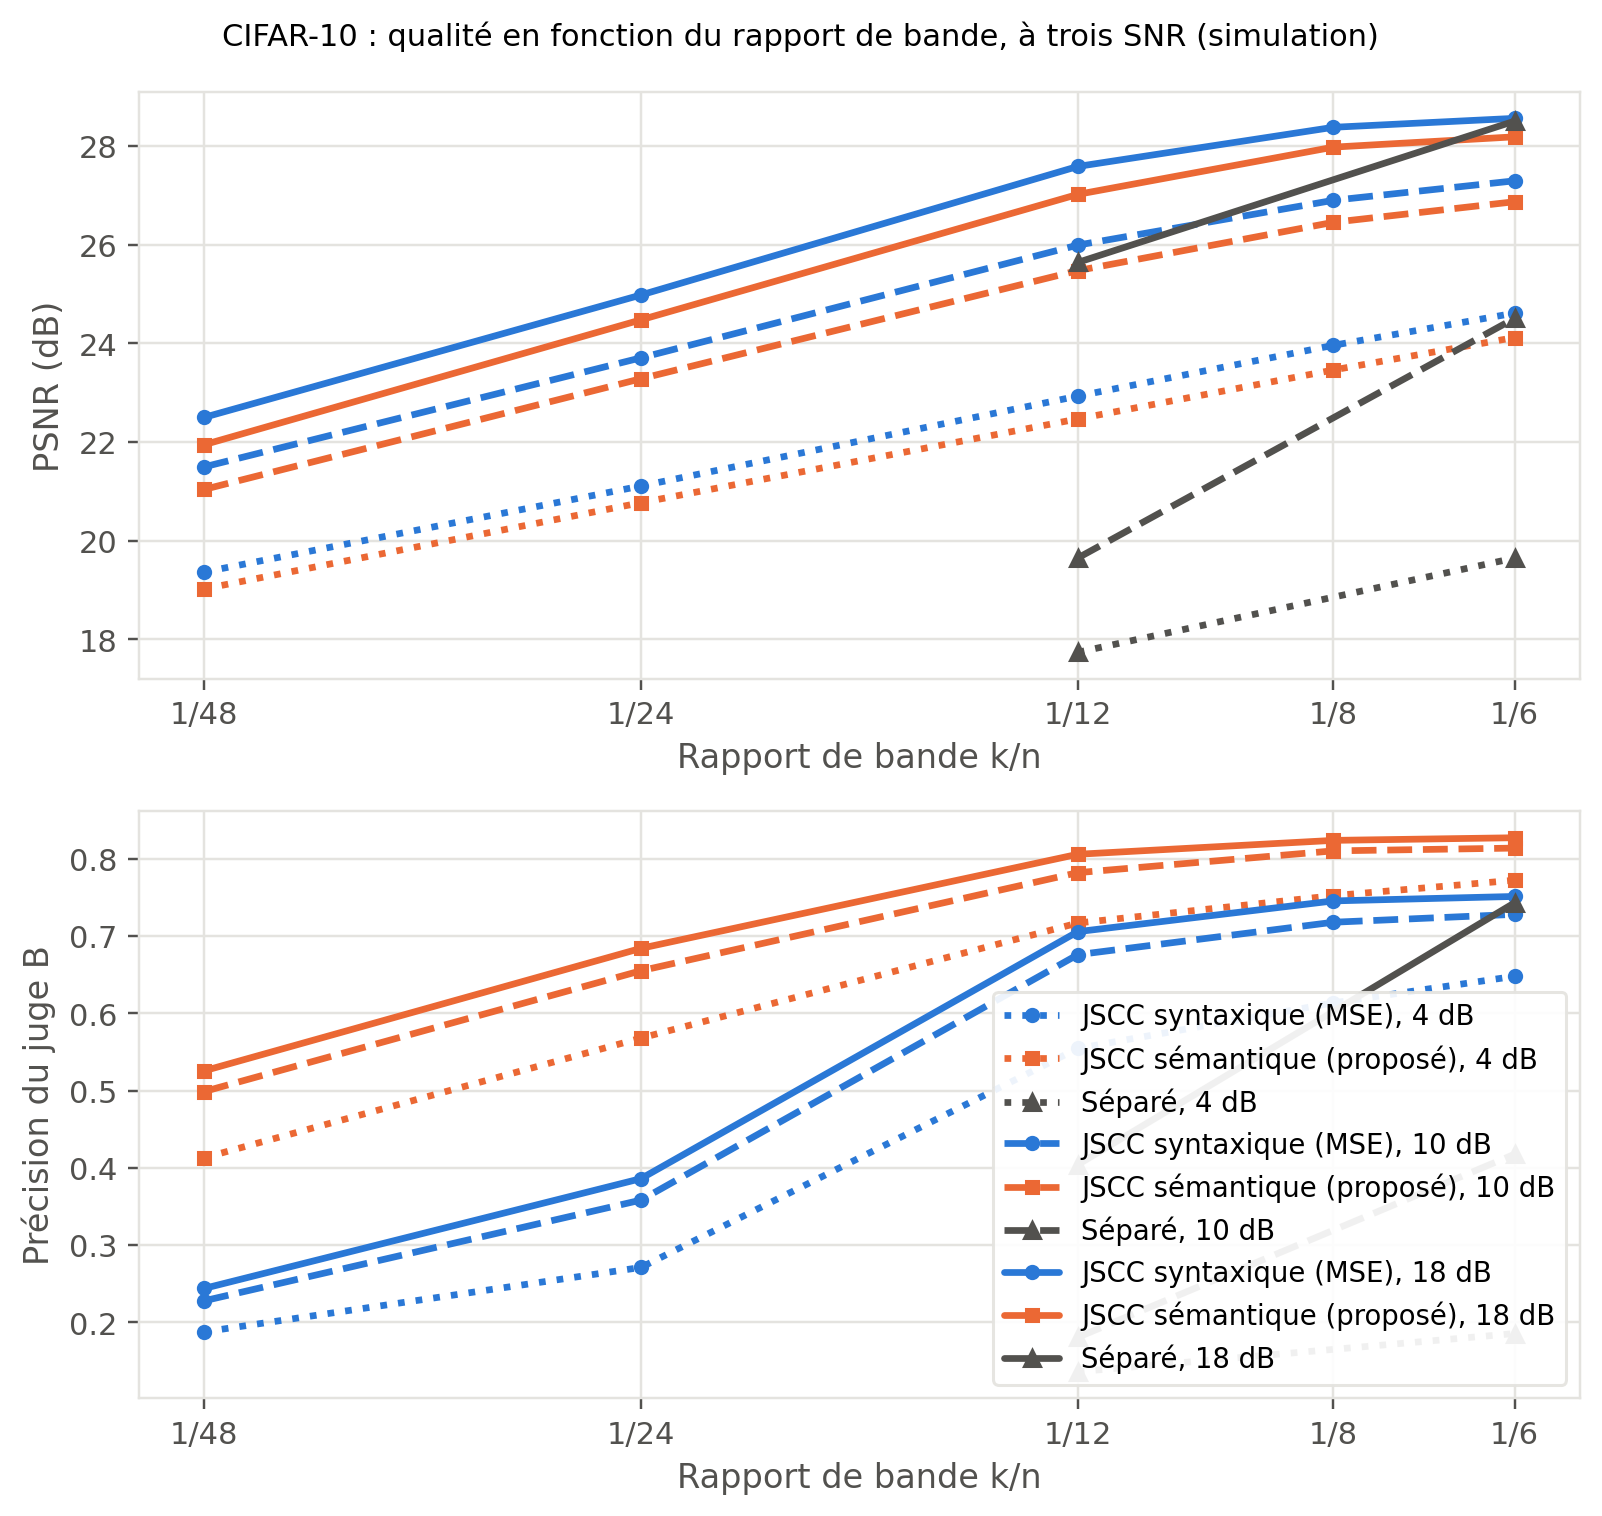
\includegraphics[width=0.96\linewidth]{cifar_bandwidth.png}
  \caption{Compromis débit/qualité sur CIFAR-10 à trois SNR. Un seul modèle couvre les cinq rapports $k/n$ ;
  les points noirs sont la chaîne séparée au meilleur MCS.}
  \label{fig:cifar_bandwidth}
\end{figure}

La chaîne séparée n'apparaît qu'aux deux budgets les plus larges : en dessous, le budget de bits ne permet
même pas un canal latent complet. À \SI{4}{\decibel} et $k/n = 1/12$, le meilleur MCS ne fait passer
qu'\emph{un seul} canal sur seize, le reste partant en redondance et en modulation prudente.

\section{Canal de Rayleigh}
\label{sec:res_rayleigh}

\begin{table}[H]
\centering
\caption{CIFAR-10 sur Rayleigh par blocs, \SI{10}{\decibel}, $k/n = 1/12$}
\label{tab:rayleigh}
\small
\begin{tabular}{@{}lrr@{}}
\toprule
\textbf{Système} & \textbf{PSNR (dB)} & \textbf{Précision} \\
\midrule
JSCC syntaxique          & 24,32 & 60,3\,\% \\
\textbf{JSCC sémantique} & 23,84 & \textbf{72,4\,\%} \\
\bottomrule
\end{tabular}
\end{table}

Même compromis qu'en AWGN — \SI{0.5}{\decibel} cédé, 12~points gagnés : le bénéfice ne dépend pas du modèle
de canal.

\begin{figure}[H]
  \centering
  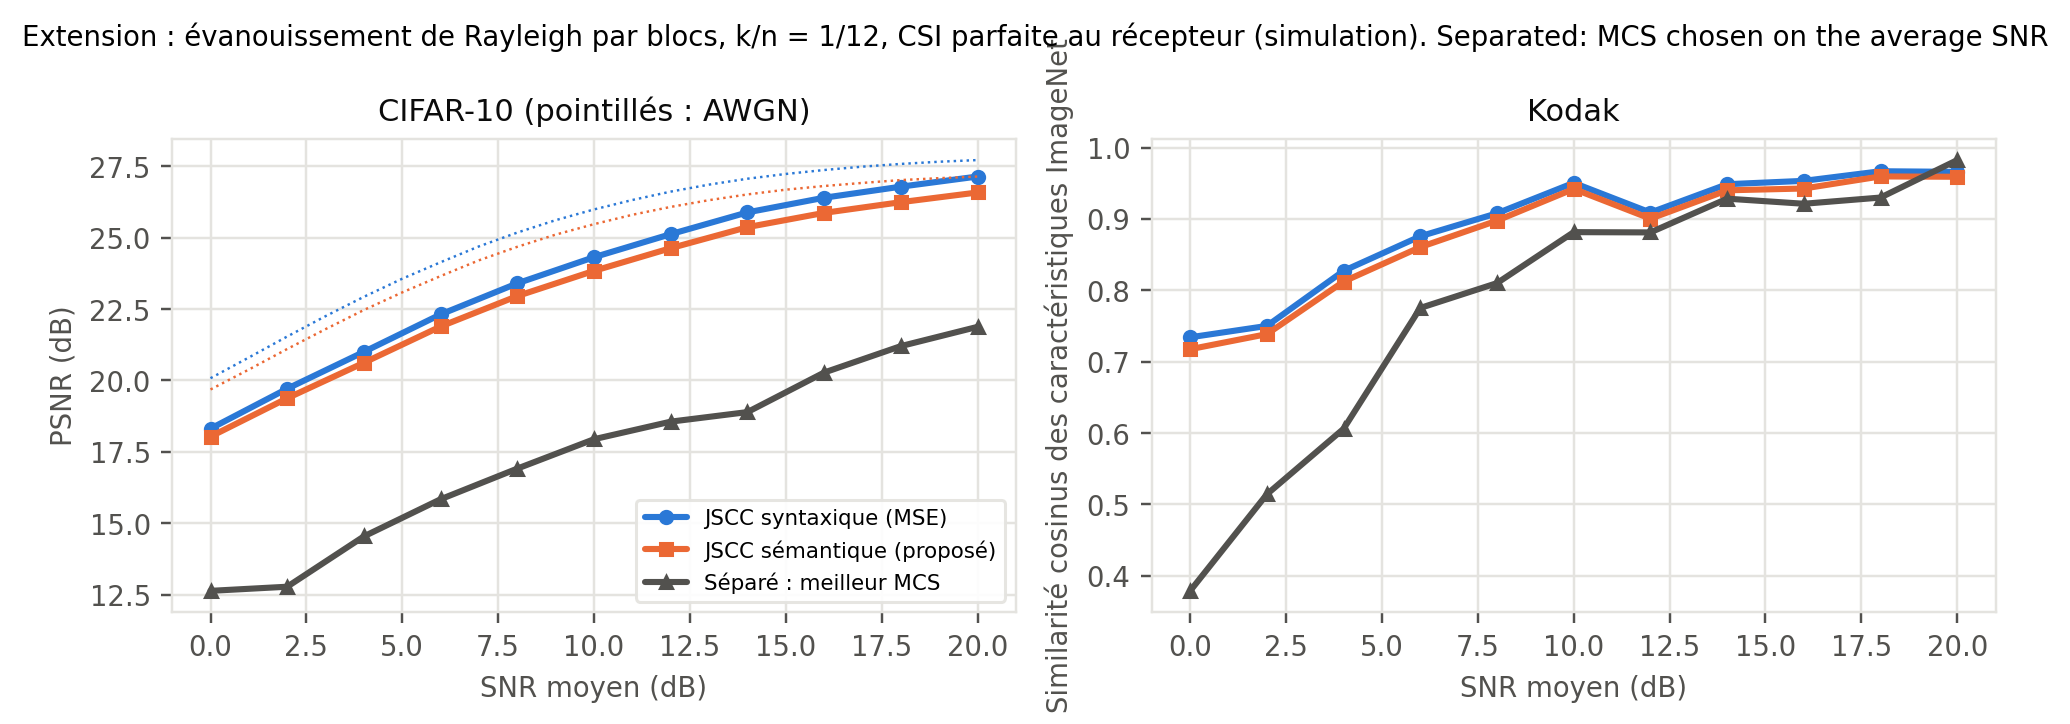
\includegraphics[width=0.94\linewidth]{rayleigh.png}
  \caption{Évanouissement de Rayleigh par blocs, CSI parfaite et égalisation par forçage à zéro.}
  \label{fig:rayleigh}
\end{figure}

\section{Désadaptation train/test du SNR}
\label{sec:res_mismatch}

\begin{table}[H]
\centering
\caption{Précision du juge B pour trois modèles entraînés à SNR fixe, $k/n = 1/12$}
\label{tab:mismatch}
\small
\begin{tabular}{@{}lrrr@{}}
\toprule
\textbf{Entraîné à} & \textbf{testé \SI{0}{\decibel}} & \textbf{testé \SI{10}{\decibel}} & \textbf{testé \SI{20}{\decibel}} \\
\midrule
\SI{0}{\decibel}  & 28,9\,\% & 30,2\,\% & 30,5\,\% \\
\SI{10}{\decibel} & 39,6\,\% & 69,5\,\% & 73,7\,\% \\
\SI{20}{\decibel} & 33,9\,\% & 67,3\,\% & 75,1\,\% \\
\bottomrule
\end{tabular}
\end{table}

Le modèle entraîné à \SI{0}{\decibel} plafonne à 30\,\% même en excellentes conditions : il n'exploite plus
la marge. Celui entraîné à \SI{20}{\decibel} s'effondre dès que le canal se dégrade. D'où la règle :
\textbf{entraîner sur une plage de SNR, jamais à un point fixe}.

\begin{figure}[H]
  \centering
  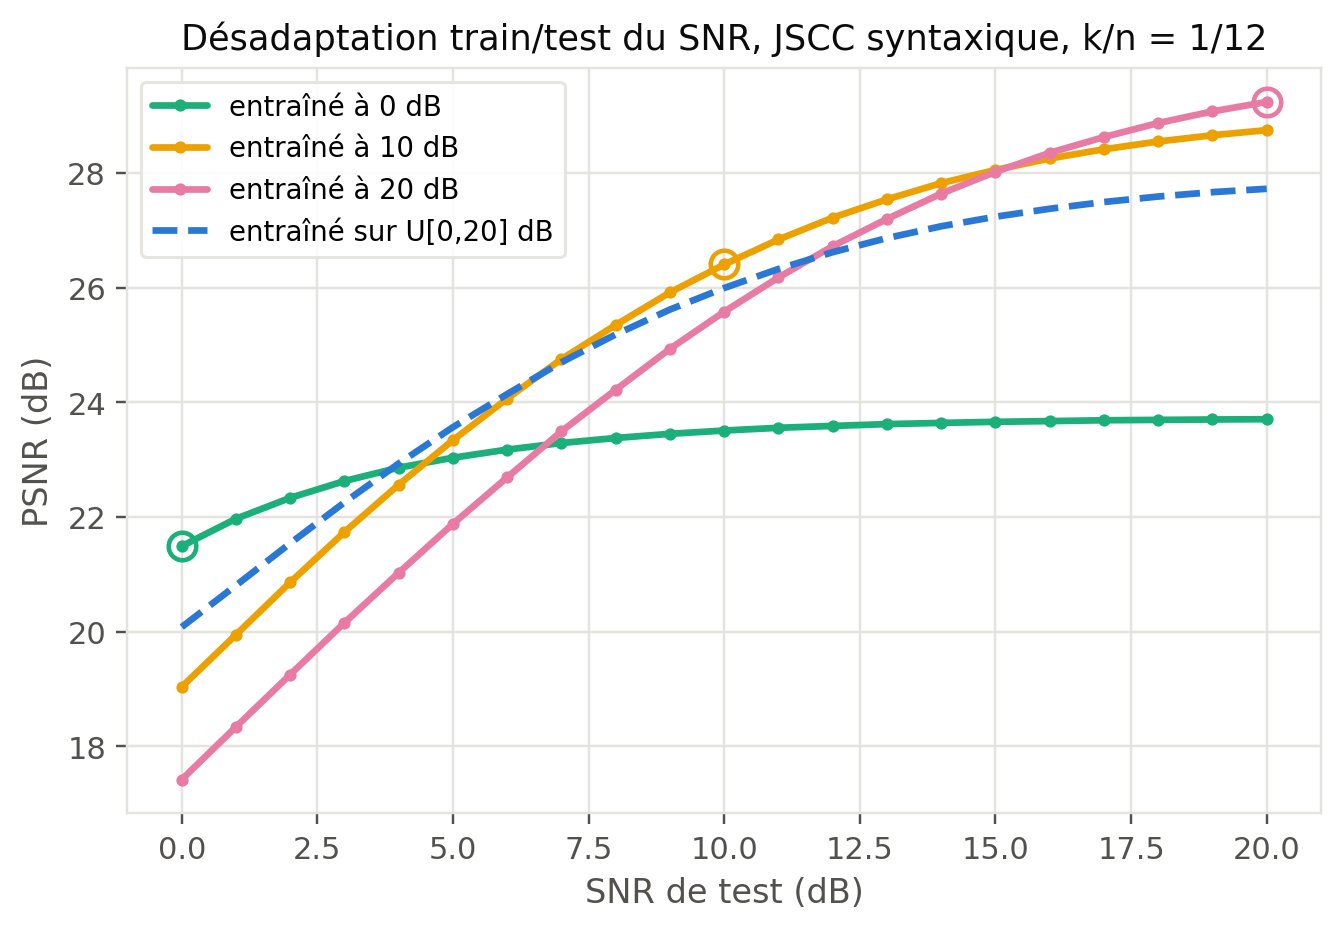
\includegraphics[width=0.88\linewidth]{snr_mismatch.png}
  \caption{Désadaptation train/test. Le cercle marque le point de conception ; la courbe en tirets est le
  modèle entraîné sur la plage complète.}
  \label{fig:mismatch}
\end{figure}

\section{Kodak et vidéo : le résultat défavorable}
\label{sec:res_kodak}

\begin{table}[H]
\centering
\caption{PSNR (dB) sur Kodak et vidéo, $k/n = 1/12$, AWGN}
\label{tab:kodak}
\small
\begin{tabular}{@{}llrrrr@{}}
\toprule
\textbf{Jeu} & \textbf{SNR} & \textbf{JSCC synt.} & \textbf{JSCC sém.} & \textbf{Séparé (capacité)} & \textbf{Séparé (meilleur MCS)} \\
\midrule
Kodak & \SI{0}{\decibel}  & 22,97 & 22,73 & \textbf{26,70} & 12,82 \\
Kodak & \SI{10}{\decibel} & 27,11 & 27,34 & \textbf{32,27} & 29,77 \\
Vidéo & \SI{0}{\decibel}  & 21,93 & 21,77 & \textbf{25,28} & 10,41 \\
Vidéo & \SI{10}{\decibel} & 26,59 & 26,62 & \textbf{31,95} & 29,11 \\
\bottomrule
\end{tabular}
\end{table}

Sur les grandes images, la borne de capacité l'emporte. Deux raisons, qu'il faut énoncer sans les atténuer :
les modèles n'ont été entraînés qu'en $32\times32$ et sont ici appliqués par transfert, terrain où JPEG est
chez lui ; et cette borne suppose zéro erreur, donc n'est pas réalisable.

Face au \emph{vrai} système séparé, la hiérarchie s'inverse dans les mauvaises conditions : à
\SI{0}{\decibel} sur Kodak, \SI{12.82}{\decibel} et 0\,\% d'accord top-1 contre $\approx$\SI{23}{\decibel}
pour les JSCC.

\begin{figure}[H]
  \centering
  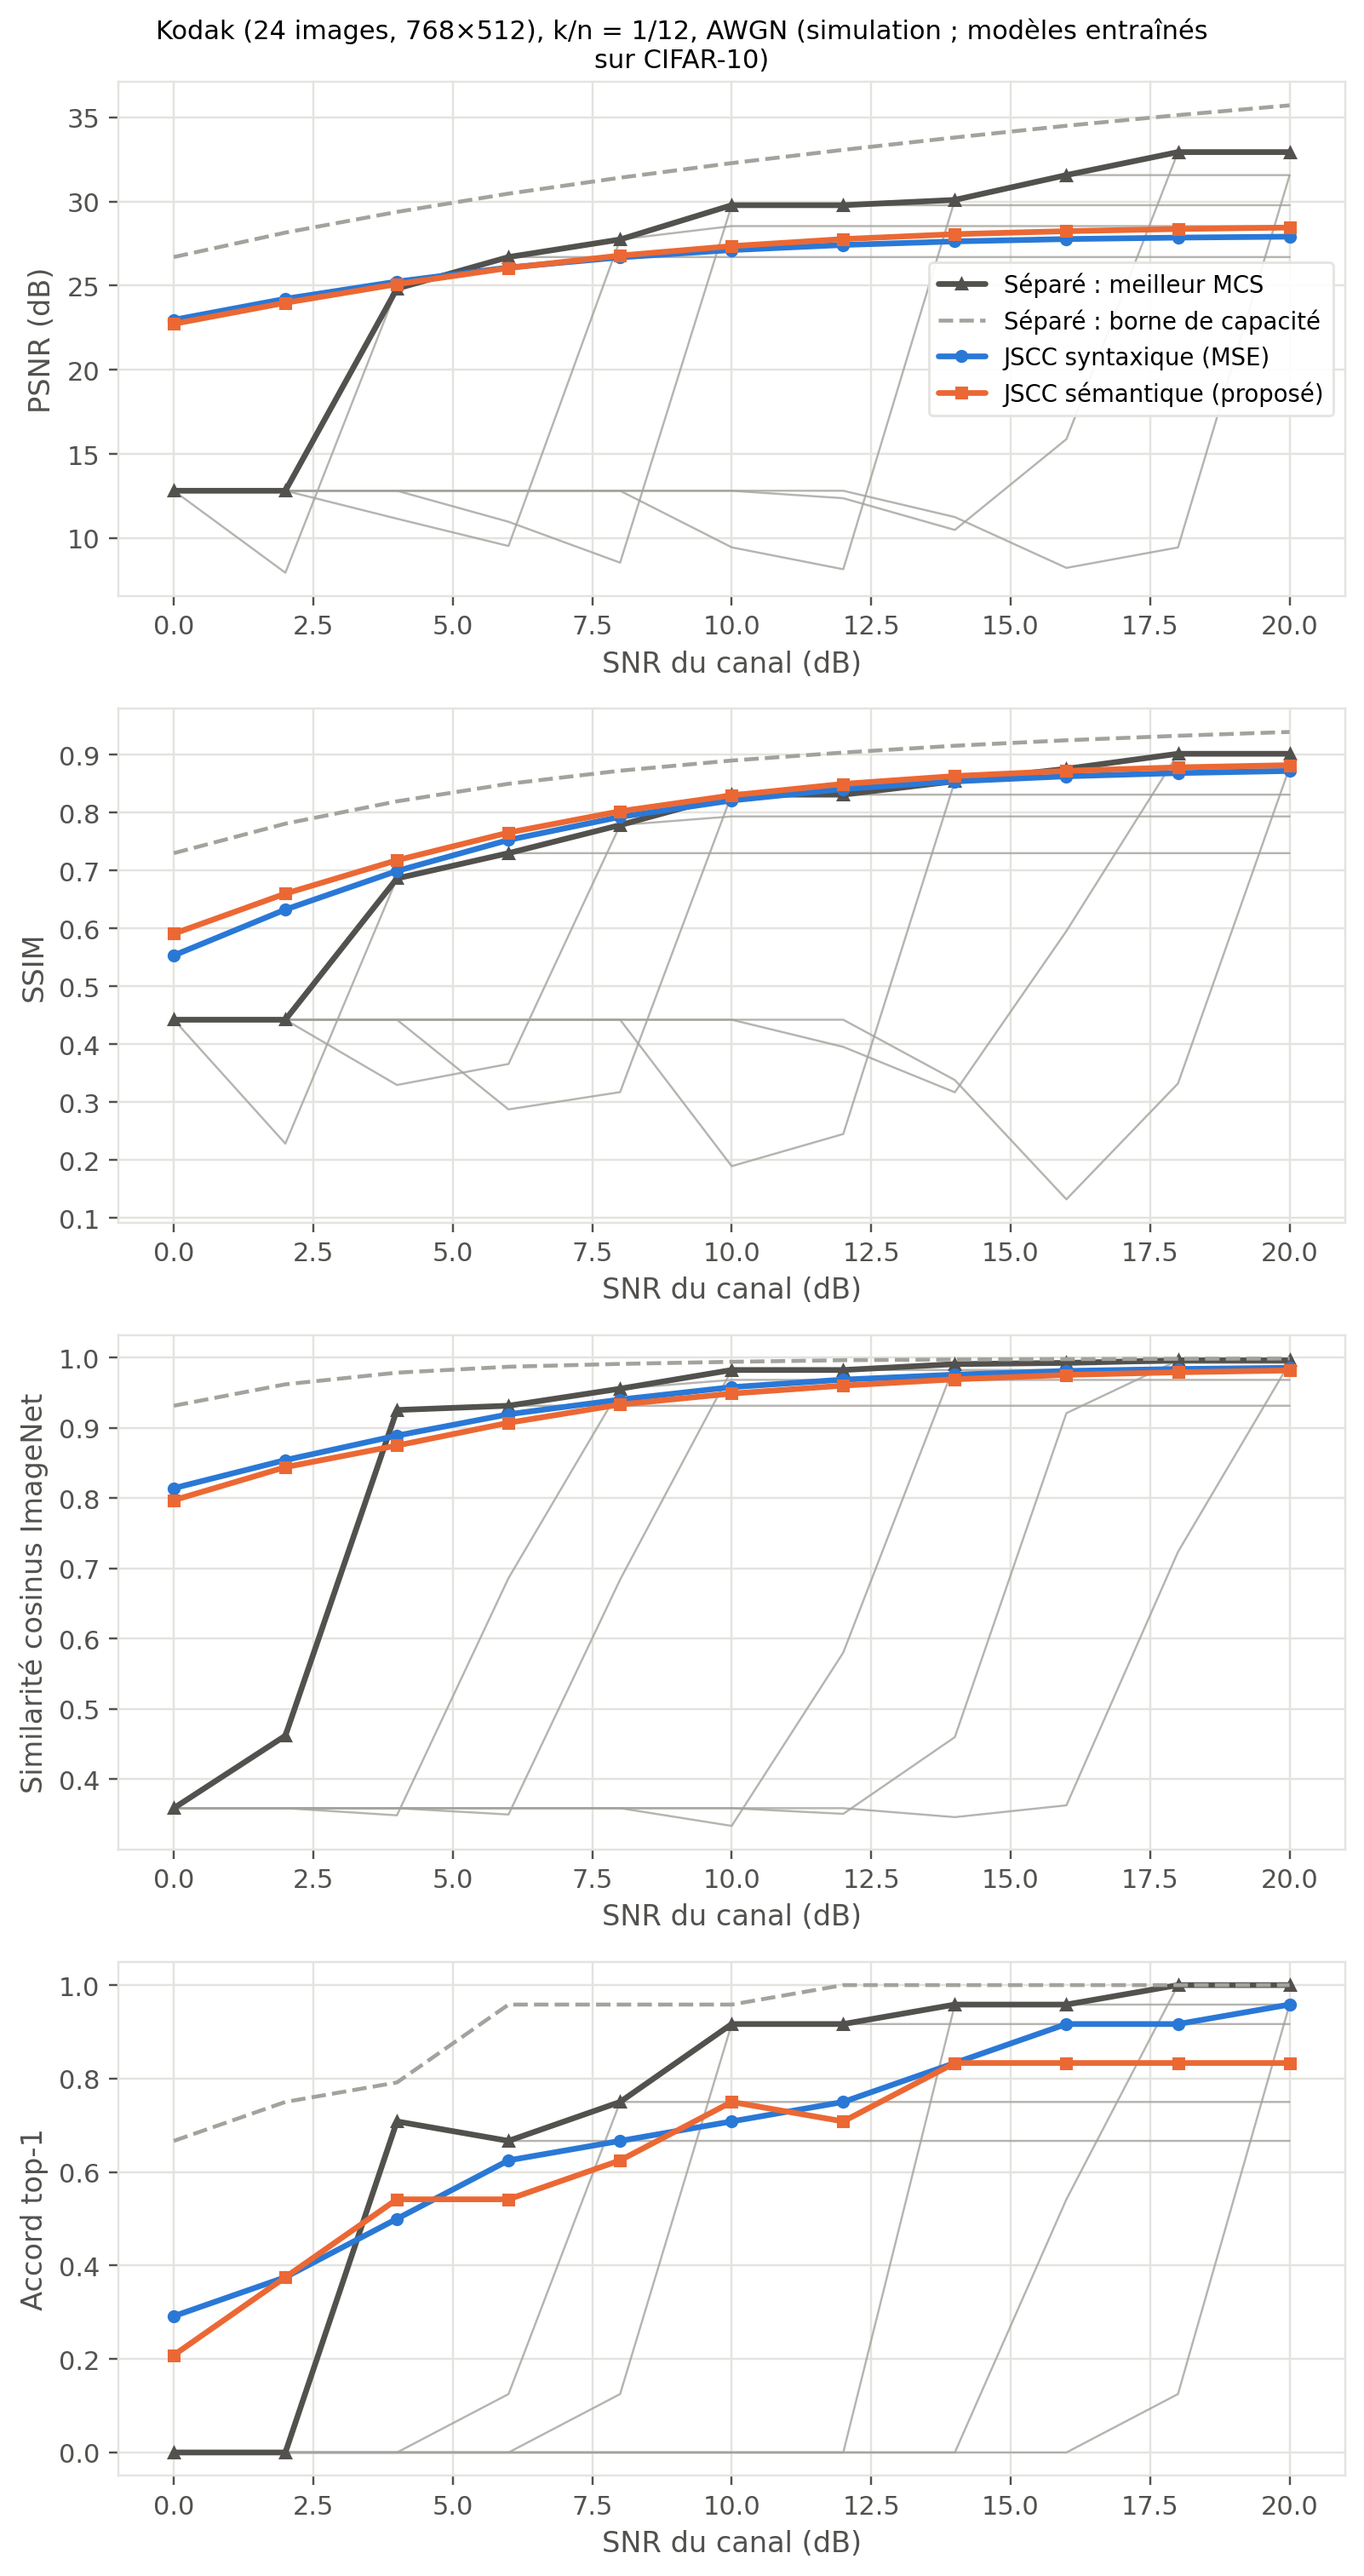
\includegraphics[width=0.76\linewidth]{kodak_snr.png}
  \caption{Kodak, 24 images $768\times512$ jamais vues à l'entraînement.}
  \label{fig:kodak}
\end{figure}

\begin{figure}[H]
  \centering
  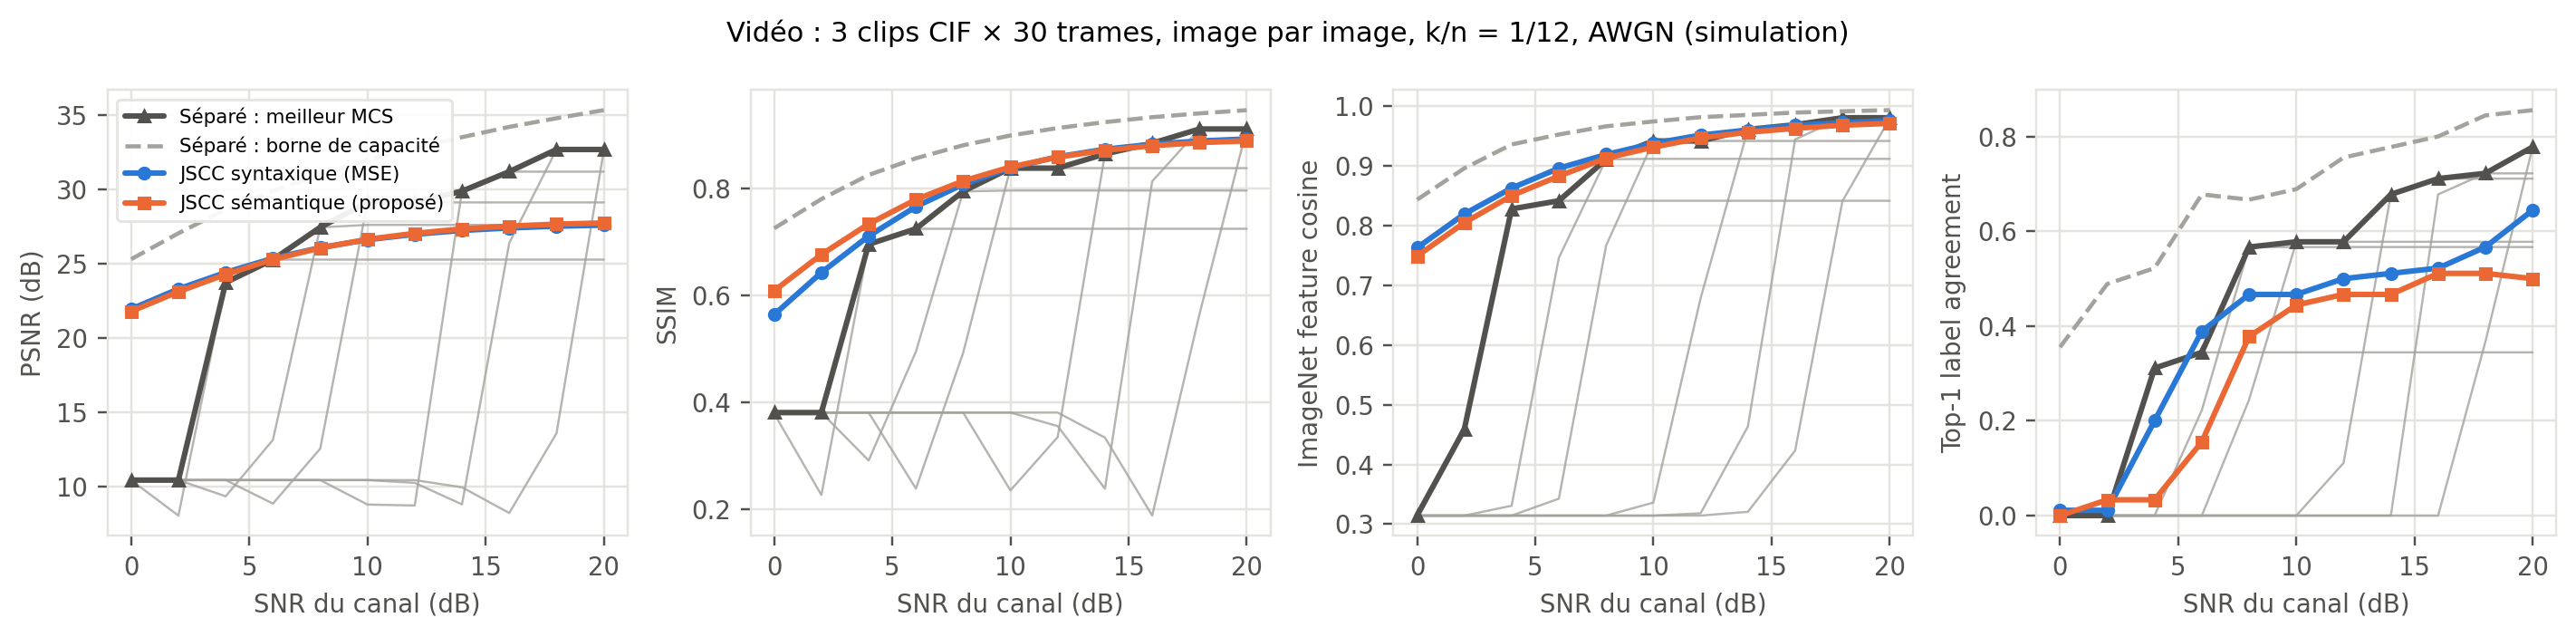
\includegraphics[width=0.76\linewidth]{video_snr.png}
  \caption{Vidéo : trois clips CIF, transmission image par image.}
  \label{fig:video}
\end{figure}

\begin{figure}[H]
  \centering
  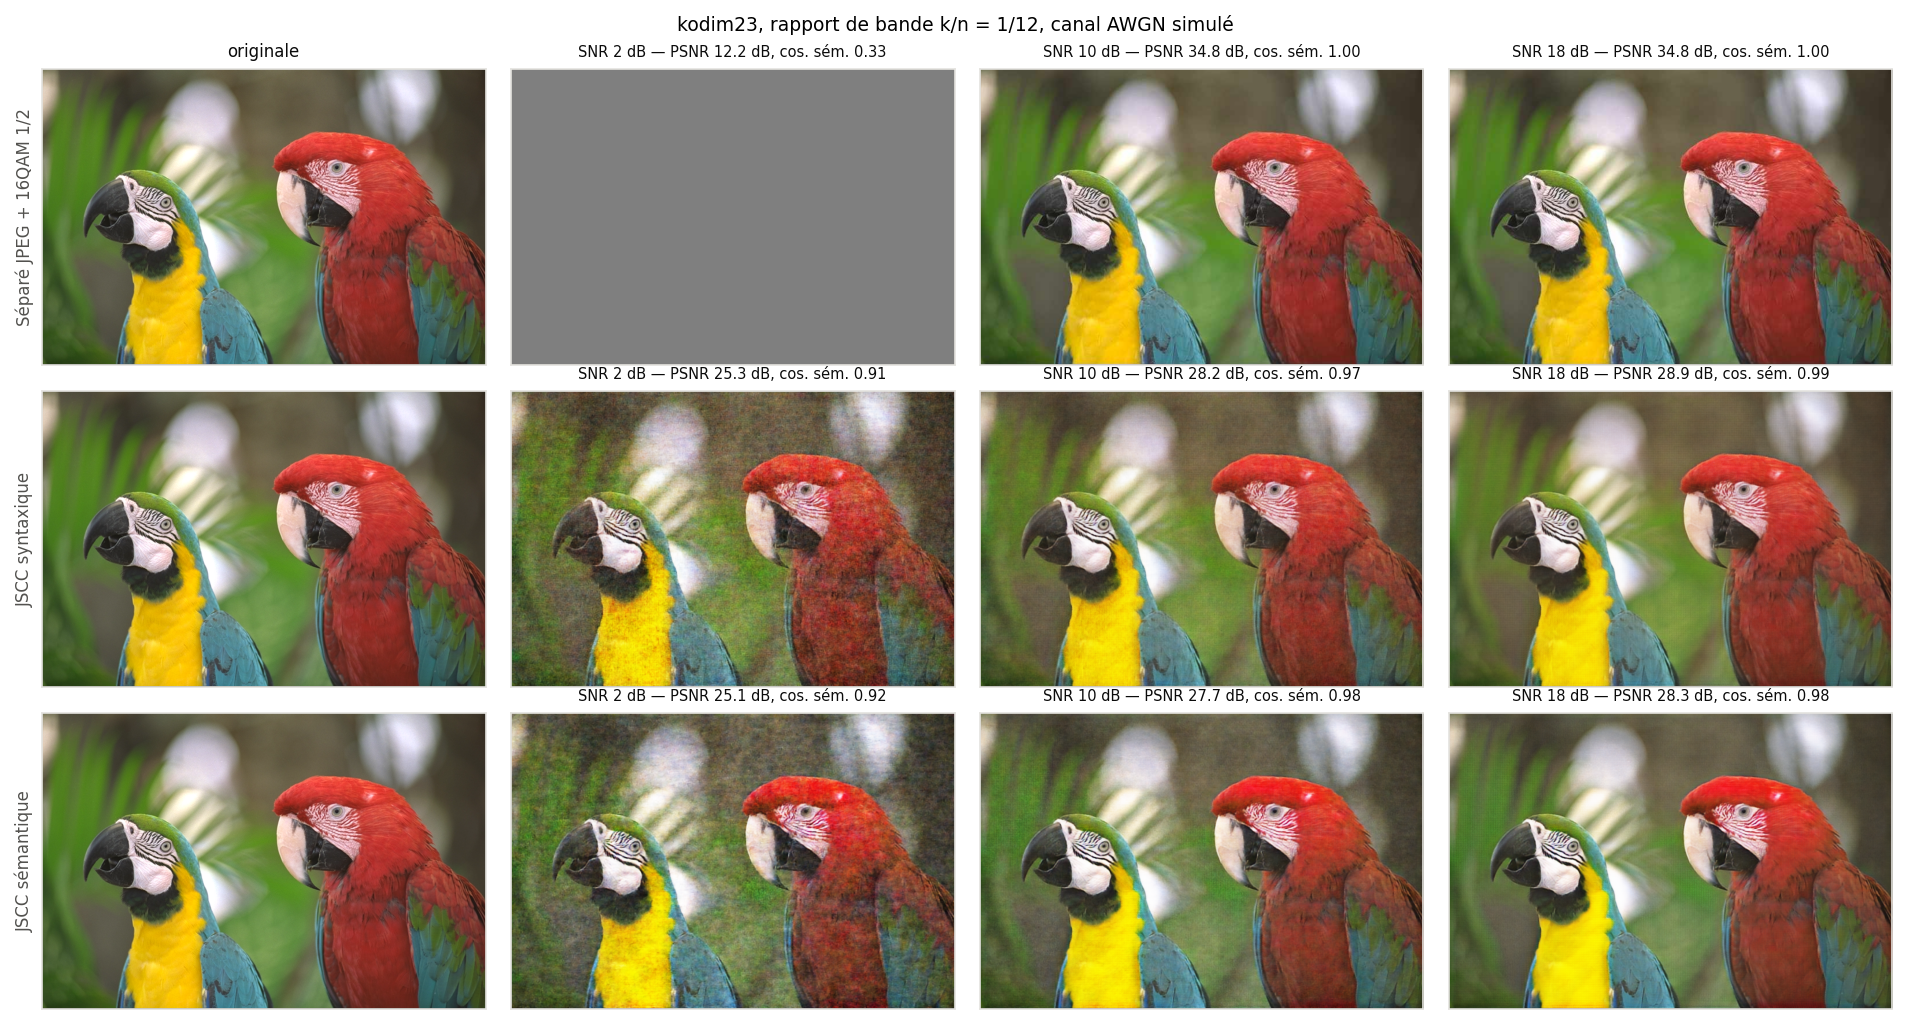
\includegraphics[width=\linewidth]{visual.png}
  \caption{Même image Kodak transmise par les trois systèmes, à trois SNR, au même budget.}
  \label{fig:visual}
\end{figure}

\section{Synthèse}
\label{sec:res_synthese}

\begin{keybox}[Ce que les mesures établissent]
\begin{enumerate}[leftmargin=1.2em]
  \item Le terme sémantique échange $\approx$\SI{0.5}{\decibel} de PSNR contre 10 à 14~points de précision,
        en AWGN comme en Rayleigh.
  \item Le codage conjoint supprime l'effet falaise.
  \item Entraîner sur une plage de SNR est indispensable.
  \item Sur grandes images non vues à l'entraînement, la borne séparée idéale reste devant en PSNR.
\end{enumerate}
\end{keybox}
